\documentclass[12pt,french, a4paper]{report}

% This is the main framework I use for my LateX documents.
% main.tex by Alexis GRACIAS

%%%%%%%%%%%%%
% LIBRARIES %
%%%%%%%%%%%%%

\usepackage{babel}
\usepackage{hyperref} % Add links to the table of content, files and website
\usepackage{graphicx} % Required for inserting images
\usepackage{tabto}
\usepackage[dvipsnames]{xcolor} % Text color package and more colors
\usepackage{tikz} % Graph package
\usepackage{pdfpages}
\usepackage{caption}
\usepackage{subcaption}
%\usepackage[demo]{graphicx}
\usepackage[utf8]{inputenc}
\usepackage{amsmath,amsfonts,mathtools,stmaryrd} % Math libraries

\usepackage{listings} % required for specific languages
\lstset{ % Set listing package options
    language=bash, % choose the language of the code
    basicstyle=\fontfamily{pcr}\selectfont\footnotesize\color{red},
    keywordstyle=\color{black}\bfseries, % style for keywords
    numbers=none, % where to put the line-numbers
    numberstyle=\tiny, % the size of the fonts that are used for the line-numbers     
    backgroundcolor=\color{white},
    showspaces=false, % show spaces adding particular underscores
    showstringspaces=false, % underline spaces within strings
    showtabs=false, % show tabs within strings adding particular underscores
    frame=single, % adds a frame around the code
    tabsize=2, % sets default tabsize to 2 spaces
    rulesepcolor=\color{gray},
    rulecolor=\color{black},
    captionpos=b, % sets the caption-position to bottom
    breaklines=true, % sets automatic line breaking
    breakatwhitespace=false, 
}

%\usepackage{eso-pic,lipsum}
%\AddToShipoutPicture{%
%	\AtTextCenter{%
%		\fboxsep5mm \fboxrule=0.8pt
%		\makebox(0,0)[c]{\fbox{\rule{0pt}\textheight\rule\textwidth{0pt}}}%
%	}%
%}

%%%%%%%%%%%%
% COMMANDS %
%%%%%%%%%%%%

\lstset{aboveskip=\baselineskip,belowskip=\baselineskip,basicstyle=\ttfamily} % Formating line break after bash commands

% Get rid of 0. chapter's number
\makeatletter 
\renewcommand{\thesection}{%
  \ifnum\c@chapter<1 \@arabic\c@section
  \else \thechapter.\@arabic\c@section
  \fi
}
\makeatother

% Rules for \bar{x} and \overline{x} commands
\makeatletter
\newcommand*{\Xbar}{}%
\DeclareRobustCommand*{\Xbar}{%
  \mathpalette\@Xbar{}%
}

\newcommand*{\@Xbar}[2]{%
  % #1: math style
  % #2: unused (empty)
  \sbox0{$#1\mathrm{X}\m@th$}%
  \sbox2{$#1X\m@th$}%
  \rlap{%
    \hbox to\wd2{%
      \hfill
      $\overline{%
        \vrule width 0pt height\ht0 %
        \kern\wd0 %
      }$%
    }%
  }%
  \copy2 %
}
\makeatother

%%%%%%%%%%%%%%%%%%%%%%
% DOCUMENTS SETTINGS %
%%%%%%%%%%%%%%%%%%%%%%
% Fist page
\title{\Huge Fiche de révision Droit}
\author{\LARGE Alexis GRACIAS}
\date{\Large \today}

% Document
\begin{document}
\maketitle
\Large \tableofcontents

%%%%%%%%%%%
% INCLUDE %
%%%%%%%%%%%

\chapter{Les normes et le raisonnement juridique}
\section{Hiérarchie des normes}
\subsection{Définition}
\large{
\textbf{Le droit} est un ensemble de \textbf{règles} qui organisent la vie en société et régissent \textbf{les relations entre les individus, les institutions et l'état.}
Ces règles sont créées par des \textbf{autorités compétentes}, comme le législateur, et sont appliquées par des tribunaux ou d'autres institutions de justice \newline

Le droit est divisé en plusieurs branches, comme : \newline

}
\begin{itemize}
    \item \textbf{Le droit civil} : concerne les relations entre les particuliers, par exemple en matière de mariage, de propriétés ou de contrats
    \item \textbf{Le droit pénal} : détermine les infractions (crimes, délits, contraventions) et fixe les sanctions applicables
    \item \textbf{Le droit administratif} : encadre les relations entre les citoyens et les administrations publiques
    \item \textbf{Le droit internationnal} : régit les relations entre les états et questions juridiques dépassant les frontières nationnales
    \item \textbf{Le droit commercial} : concerne les activités économiques, les entreprises et les transactions commerciales
\end{itemize}
En cas de non respect de ces règles, le citoyen encours des sanctions. Le droit peut évoluer dans le temps en fonction des changements sociaux, technologiques ou économiques
\begin{center}
    \begin{figure}[hbt!]
        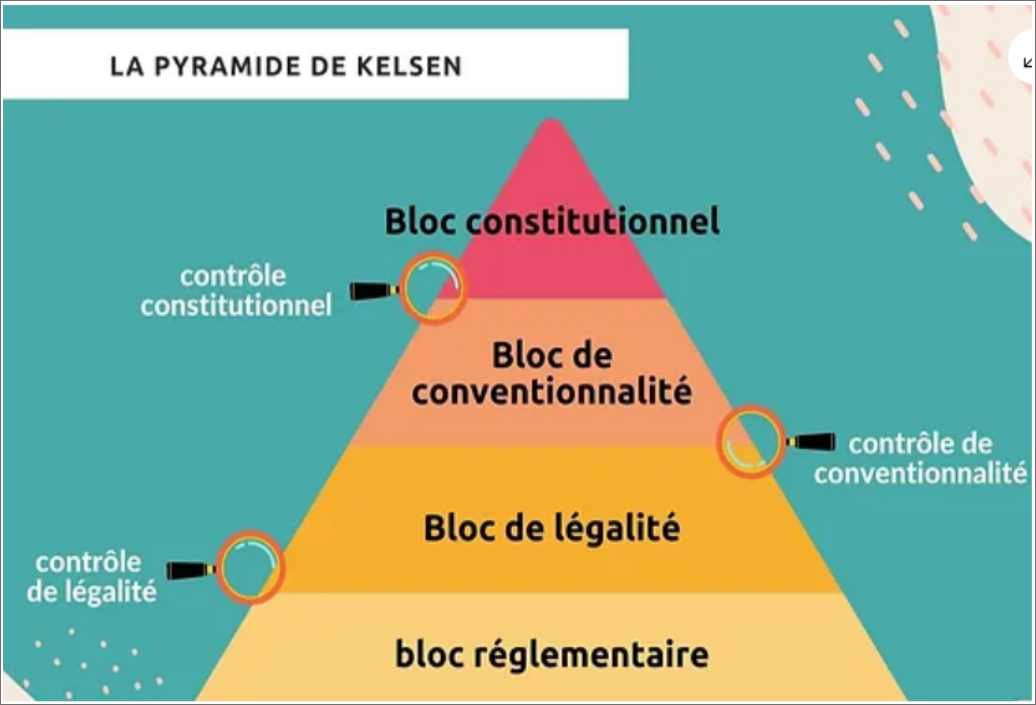
\includegraphics[scale=0.4]{Pics/Pyramide_de_Kelsen.png}
        \caption{Hiérarchie des normes}
    \end{figure}
\end{center}
\newpage
\section{Les normes}
Les \textbf{normes juridiques} sont à différentier des \textbf{normes sociales}. Une norme juridique est une règle qui établit une source de droits et d'obligations juridiques tandis
qu'une norme sociale provient d'une tradition, de la morale lorsqu'un individu se socialise. 
\subsection{Bloc constitutionnel}
C'est la Constitution : un ensemble de normes juridiques, de principes et de règles appliquées par le conseil constitutionnel. \footnote{Vérifie la conformité des lois à la Constitution}
\begin{center}
    \begin{figure}[hbt!]
        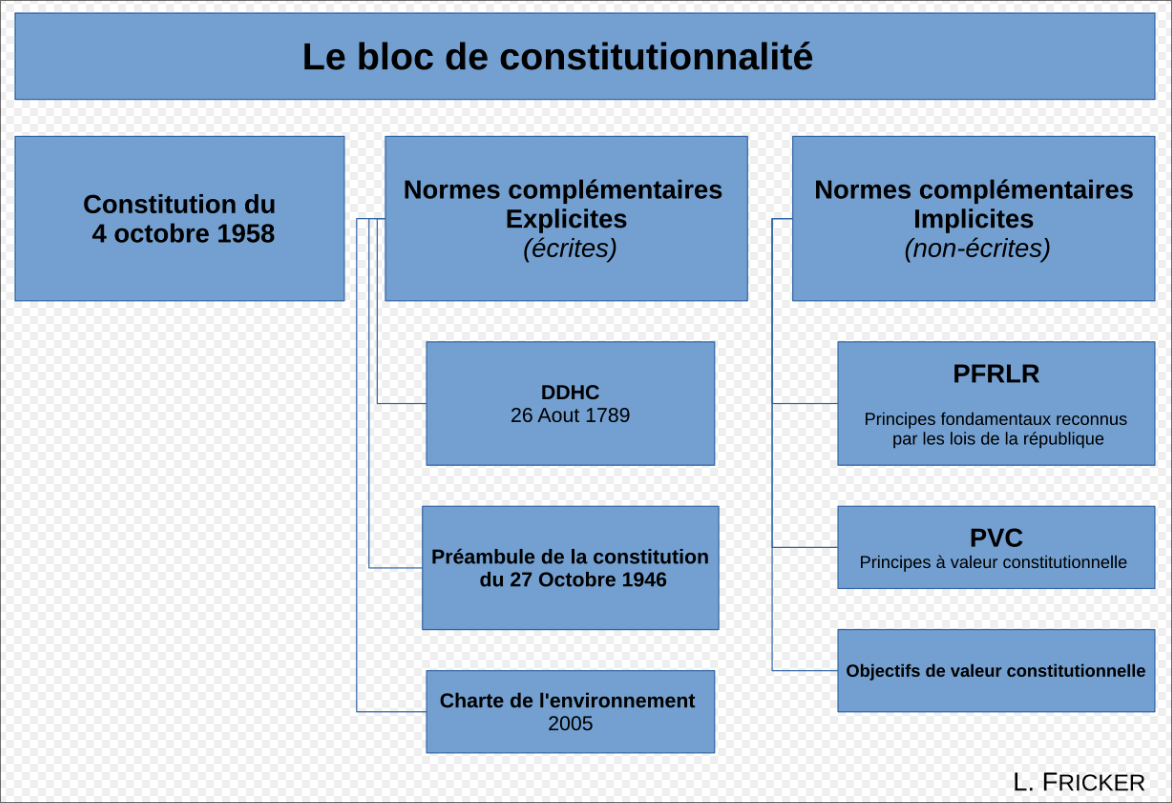
\includegraphics[scale=0.3]{Pics/Bloc_de_constitutionnalite.png}
        \caption{Bloc constitutionnel}
    \end{figure}
\end{center}
\newpage
\subsection{Bloc conventionnel}
\textbf{Le bloc de conventionnalité l'ensemble des traités et conventions entre les Etats ou entre mes Etats et les organisations internationnales} \newline
Exemple : l'\textbf{UE} est une organisation économique et politique qui rasssemble 27 états membres. Elle a pour but de promouvoir la paix, la stabilité et la coopération économique entre les états memebres. \newline
\begin{center}
    \begin{figure}[hbt!]
        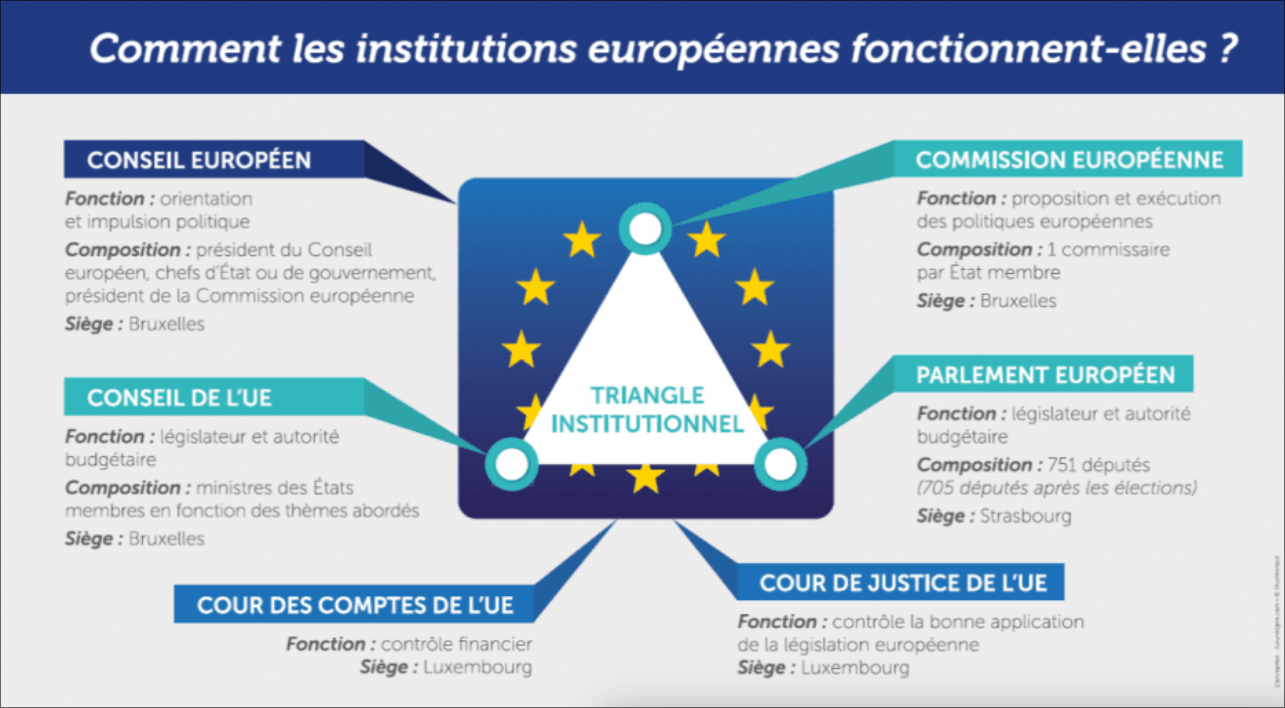
\includegraphics[scale=0.3]{Pics/Institutions_UE.png}
        \caption{Illustration des institutions dans l'Union Européenne}
    \end{figure}
\end{center}
\newpage

\chapter{Les contrats vus à travers l'énergie}
\section{Le Fonctionnement des marchés de gros de l'électricité}
\subsection{L’organisation de l’opérateur historique avant la libéralisation}
\begin{figure}[hbt!]
    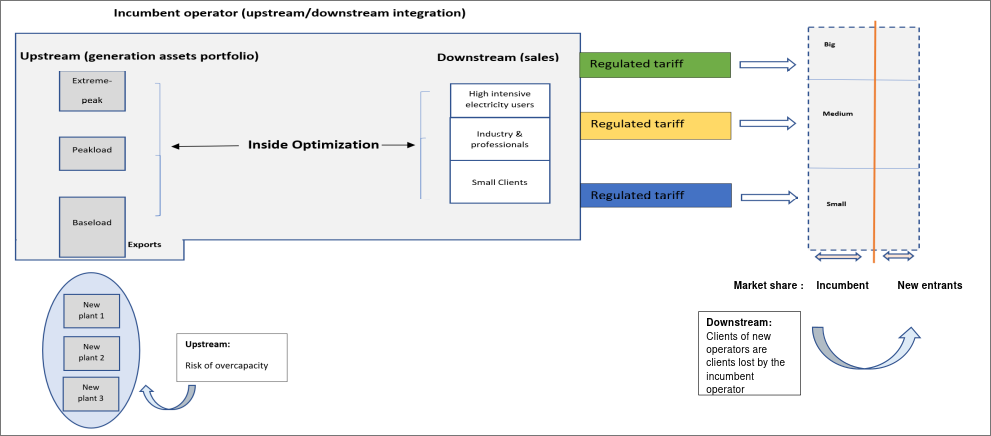
\includegraphics[scale=0.4]{Pics/marche_de_l_electricite_avant_liberalisation.png}
\end{figure}
\newpage
\subsection{Les business models}
\subsubsection{Stand alone model}
Modèle ou les fournisseurs d'électricité sont indépendants du réseau principal. Ce business model est conçu pour fonctionner dans des endroits isolés. Exemple d'UEM pour le réseau de Metz. \newline
C'est le modèle qu'a adoptée la commisison en 2007 pour les marchés de gros.
\begin{figure}[hbt!]
    \centering
    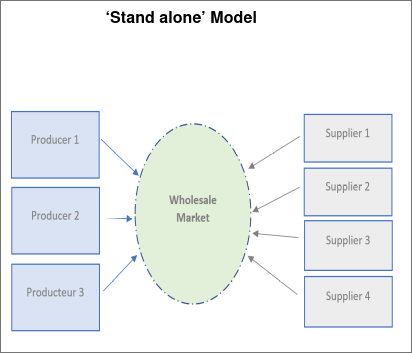
\includegraphics[scale=0.7]{Pics/Stand_alone_model.png}
\end{figure}
\newpage
\subsubsection{Fully Integrated Utilities}
Services publics entièrement intégrés. L'opérateur assure toute la chaine d'approvisionnement de l'électricité de manière centralisée, de la production jusqu'à la distribution aux clients finaux. S'oopose aux modèles fragmentés ou les différents segments sont réalisés par différentes entités.
\begin{figure}[hbt!]
    \centering
    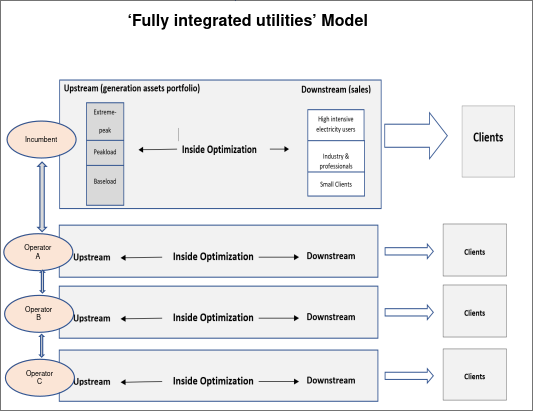
\includegraphics[scale=0.7]{Pics/Fully_integrated_model.png}
\end{figure}
\newpage
\section{La crise des prix pour le marché de gros de l'électricité}
Ordre de mérite :
\begin{figure}[hbt!]
    \centering
    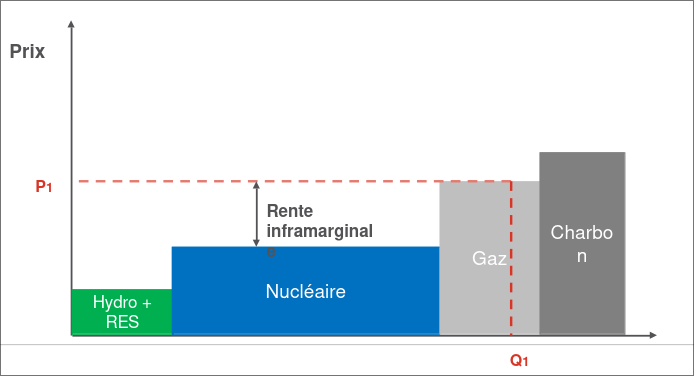
\includegraphics[scale=0.5]{Pics/ordre_de_merite.png}
\end{figure}
\begin{figure}[hbt!]
    \centering
    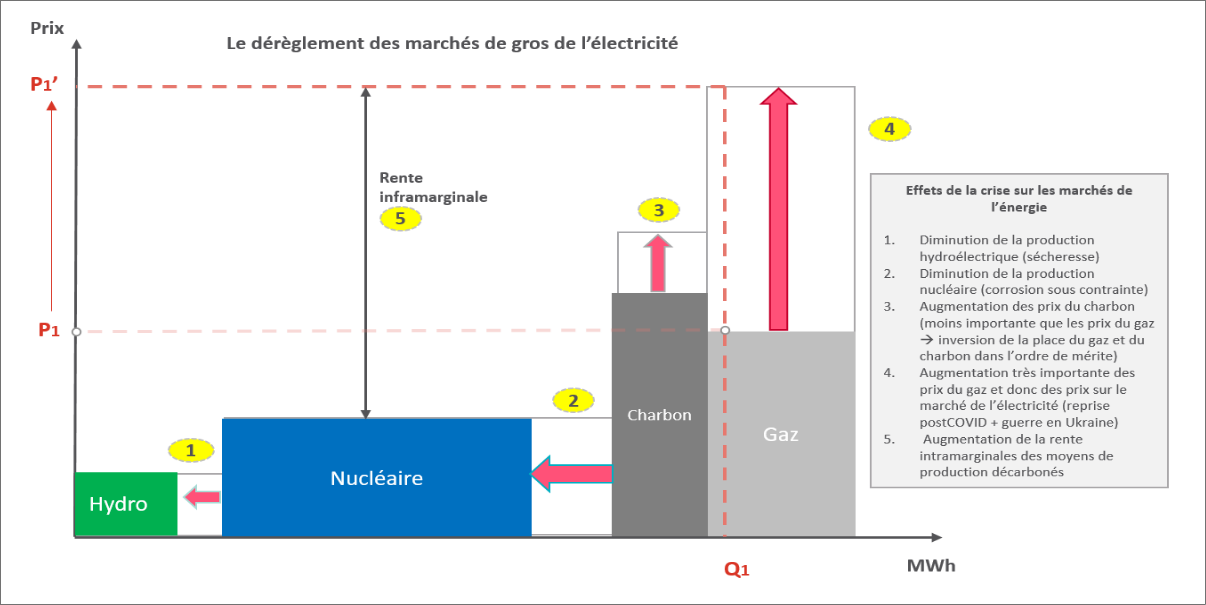
\includegraphics[scale=0.35]{Pics/dereglement_prix_elec.png}
\end{figure}
\newpage
\begin{figure}[hbt!]
    \centering
    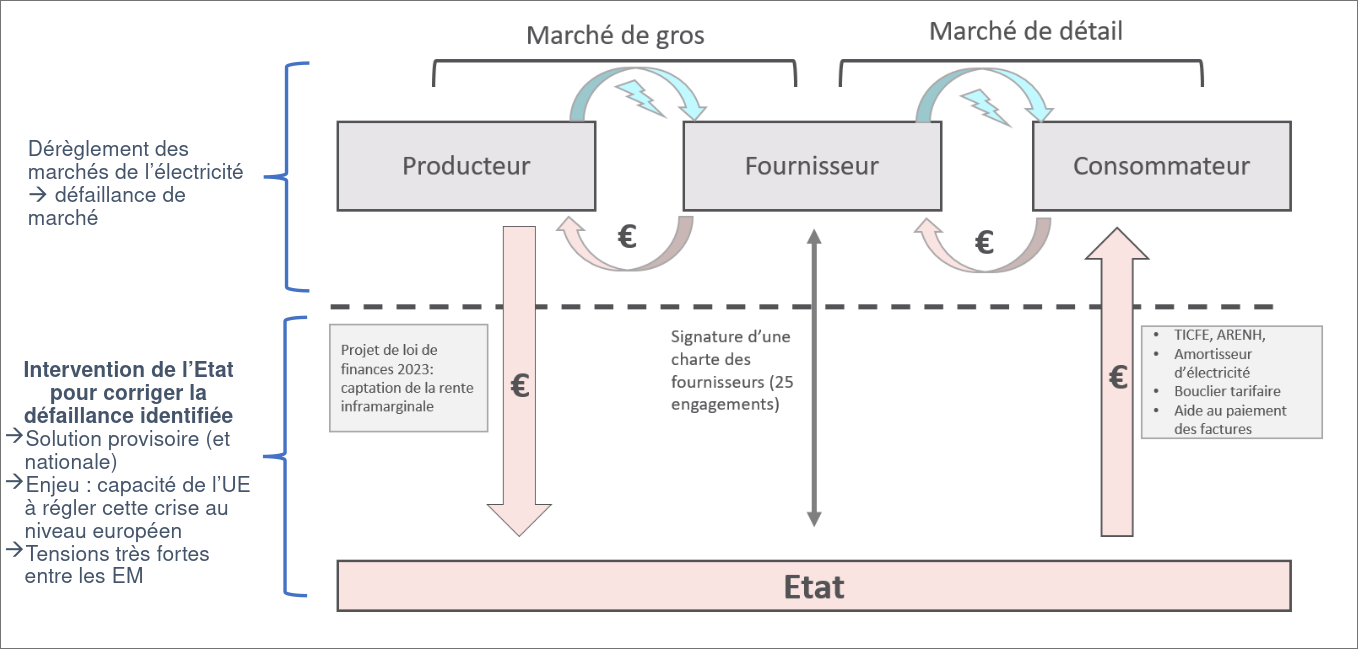
\includegraphics[scale=0.3]{Pics/fiscalite_et_surprofits.png}
\end{figure}
Solutions mises en place pour la protection des consommateurs sur la hausse des prix :
\begin{itemize}
    \item Règlement du conseil de l'UE \footnote{Article 6: 1. « Les recettes issues du marché obtenues par les producteurs d’électricité à partir des sources visées à l’article 7, paragraphe 1, sont plafonnées à un maximum de 180 EUR par MWh d’électricité produite ».}
    \item Loi n°2022-1726 du 30 décembre 2022 : \textbf{loi de finance pour 2023} en France $\implies$ \textbf{Article 54} \newline
\end{itemize}
Fonctionnement de l'article 54 : 
\begin{figure}[hbt!]
    \centering
    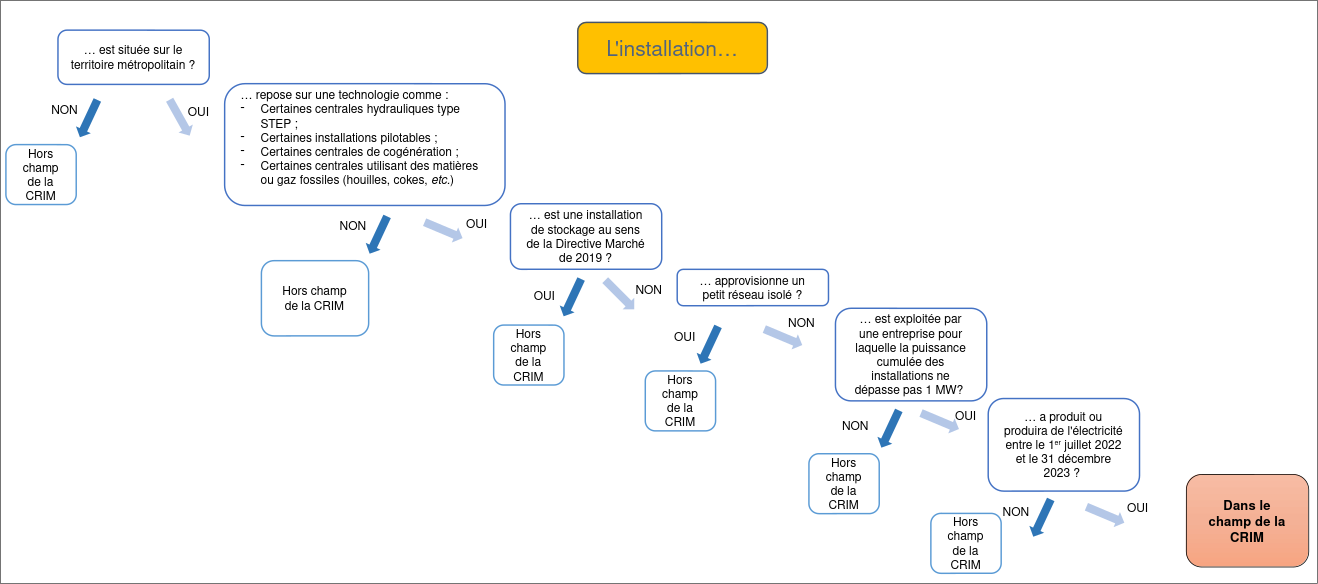
\includegraphics[scale=0.3]{Pics/principe_art_54.png}
\end{figure}
\newpage
« Le montant de la contribution est égal à la fraction des revenus de marché de l'exploitant de l'installation excédant un seuil forfaitaire. Cette fraction fait l'objet d'un abattement de 10 \% »
\begin{center}
    \Large{\fbox{$
    MF = Rm - F - D
    $}}
\end{center}
\begin{itemize}
    \item $MF$ : marge forfaitaire
    \item $Rm$ : revenu de marché
    \item $F$ : forfait
    \item $D$ : déductions finales
\end{itemize}
\section{Fiscalité en market design}
Proposition de la commisison E de réformer le Fonctionnement de marché de gros (2023) : \newline
Il y a des problèmes :
\begin{itemize}
    \item Centralisation excessive du larché de gros à court terme
    \item Potection des consommateurs de la volatilité des prix à court terme
    \item Discussions sur les contrats long terme : ils étaient jusqu'alors perçus comme des freins à la libéralisation du secteur de l'électricité
\end{itemize}
\newpage
\section{Les contrats long terme}
\subsection{Les CFD (contract for difference)}   
C'est un contract entre un investisseur et un courtier : l'investisseur spécule sur la hausse ou la baisse d'un bien. Si la valeur du bien augmente, le courtier paye la différence de prix entre le début et la fin du contrat. Si la valeur du bien diminue, c'est l'investisseur qui compense.
\begin{figure}[hbt!]
    \centering
    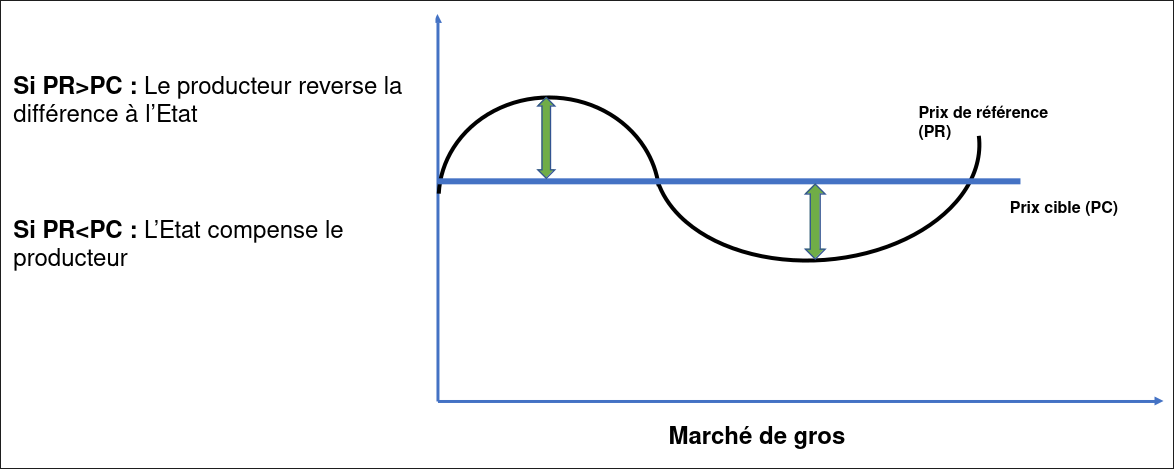
\includegraphics[scale=0.3531]{Pics/CFD_fonctionnement.png}
\end{figure}
\subsection{Les PPA (Power Purchase Agreement)}
C'est un contrat entre un client et un fournisseur d'électricité. Le fournisseur s'engage à produire une certaine quantité d'énergie pendant que le client s'engage à payer une certaine somme, correspondant à cette quantité d'énergie indexée sur le prix de l'électricité ou bien un prix fixe. Si le marché fluctue, ils compensent la différence.
\newpage
\begin{figure}[hbt!]
    \centering
    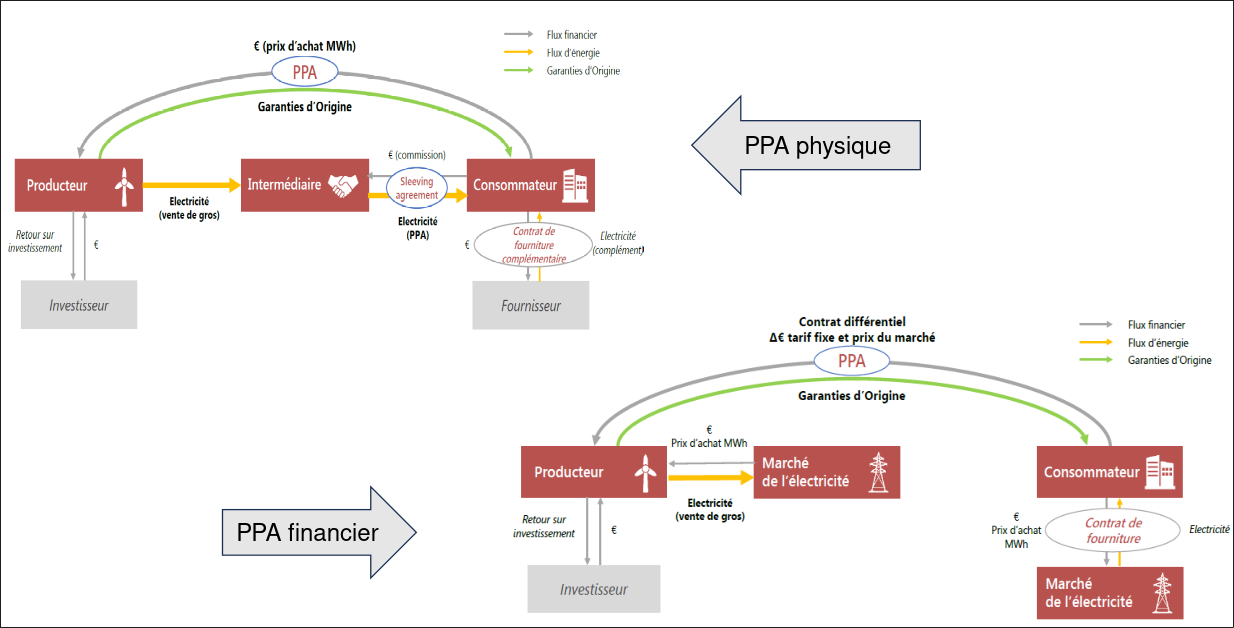
\includegraphics[scale=0.3531]{Pics/PPA_physique_et_PPA_financier.png}
\end{figure}
\subsection{Risk sharing contract}
Contrat de partage de risques. Les écarts entre la consommation cible sont compensés par les deux parties (consommateur et fournisseur). Ces parties peuvent êtres inégales. Par exemple : quand la consommation est trop grande par rapport à la cible, le client paye $2/3$ de l'écart et $1/3$ pour le fournisseur. A l'inverse, si la cible est surévaluée et le consommateur consomme finalement moins que la cible, le fournisseur rembourse $4/5$ de la différence.
\subsection{Purely supply contract}
Contrat de fourniture pure. L'approvisionnement de l'énergie est purement définie, c'est-à-dire qu'une quantité d'énergie est délivrée et payée, sans considérer la part de risques, car il n'y a pas de cible prévisionnelle : uniquement une quantité payée et effectivement consommée.
\newpage
\section{Liquidité des marchés de gros}
\textbf{Liquidité : facilité de vendre et d'acheter une grosse quantité d'électricité sans affecter les prix du marché.} Le manque de liquidité cause une volatilité conséquente \footnote{Taux de variation des prix en fonction du temps} \newline
Les PPA ne sont pas la bonne solution pour la liquidité, c'est pour cela que la Commisison Européenne favorise le stand-alone model. Cependant, le modèle du stand-alone force le marché de gros, qui lui-même est un marché très volatile \footnote{problèmes de stockage liés à l'énergie électrique}. De plus, le stand-alone model n'es pas optimal d'un point de vue industriel et colectif \footnote{Rapport Champsaur}. Il faut alors que la Commisison se penche sur d'autres modèles que le stand alone : il ne doit pas être le seul modèle.
\section{La nécéssité d'évolution dans l'appréciation des contrats long terme pour la Comission}
\begin{figure}[hhbt!]
    \centering
    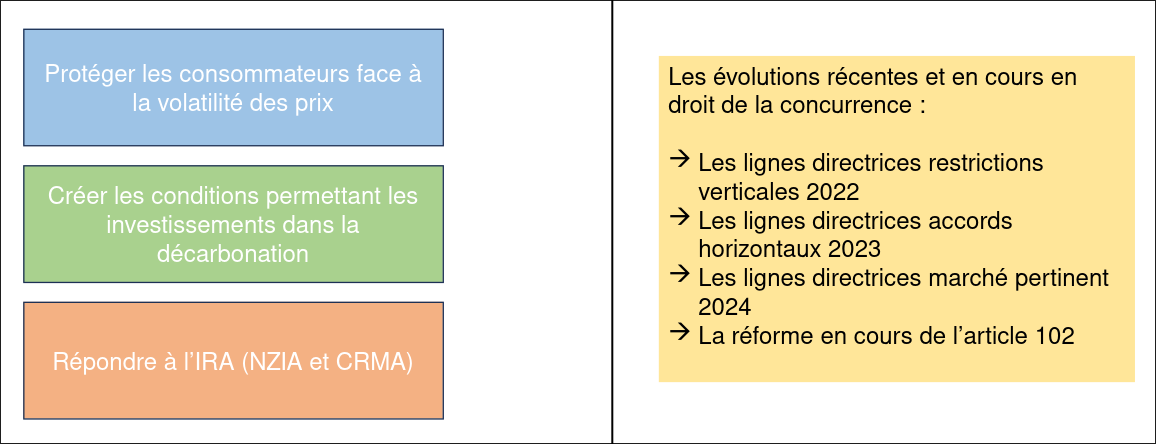
\includegraphics[scale=0.35]{Pics/evolution_contrat_long_terme.png}
\end{figure}
\chapter{Les grandes tendances du droit}
\section{Les contentieux climatiques}
\subsection{L’affaire Grande-Synthe}
\begin{itemize}
    \item CE 19 nov. 2020, n° 427301, Grande-Synthe (Cne)
    \item CE 1er juill. 2021, n° 427301, Grande-Synthe (Cne)
    \item CE, ass., 10 mai 2023, n° 467982,  Grande Synthe
\end{itemize}
\subsection{Le conseil d'état}
Présidé par le premier ministre et à son vice-président
Le conseil d'état a deux grandes missions : \footnote{Les ordres administratifs et judiciaires sont séparés en France}
\begin{itemize}
    \item \textbf{Conseiller le gouvernement} : préparation des lois, ordonnances, certains projets et décrets. \textbf{La cour de cassation est la plus haute entité judiciaire}
    \item \textbf{Juge administratif suprême} : juge les litiges entre l'administration et les administrés, c'est \textbf{la plus haute entité administrative}
\end{itemize}
\newpage
\subsection{Les sections consultatives}
Examination des projets de loi, plusieurs sections :
\begin{itemize}
    \item Section de la \textbf{finance}
    \item Section de l'\textbf{intérieur}
    \item Section \textbf{sociale}
    \item Section des \textbf{travaux publics}
    \item Section de l'\textbf{administration}
\end{itemize}
Les décisions urgentes sont prises par la \textbf{commisison permanente}
\subsection{La section du contentieux}

\chapter{Annexe sur les institutions de l'UE et ses principes}
\newpage
\section{L'UE et ses institutions}
Exemple de traités fondateurs :
\begin{itemize}
    \item Communauté Européenne de charbon et de l'acier (CECA) 1951 qui réunit les pays fondateurs de l'UE : l'Allemagne, l'Italie, la France, le Luxembourg, les Pays Bas et la Belgique
    \item Communauté Economique Européenne (CEE), traité de Rome 
    \item Communauté Européenne de l'Energie Atomique (EURATOM), 1957 \newline
\end{itemize}

Institutions principales : 
\begin{itemize}
    \item La commission européenne : propose les lois et veille à leurs applications
    \item Le parlement européen : représente la voix des citoyens
    \item Le conseil de l'UE : représente les Etats et co-légifère avec le parlement
    \item Le conseil Européen : réunion des chefs d'Etat pour donner les orientations politiques
    \item La cour de justice de l'UE : veille à l'interprétation et l'application du droit européen \newline
\end{itemize}

\newpage
Politiques clés :
\begin{itemize}
    \item Le climat
    \item La sécurité
    \item Les droits sociaux et l'égalité \newline
\end{itemize}

Traités :
\begin{itemize}
    \item Traité sur l'UE
    \item EURATOM
    \item \textbf{Traité sur le Fonctionnement de l'Union Européenne (TFUE)} \newline
\end{itemize}
\newpage
\section{Principe de subsidiarité}
Permet de déterminer le niveau d'intervention le plus pertinant des états membres pour la mise en place des actions envisagées
\newline
\section{Compétences partagées}
Les états membres de l'UE peuvent partager leurs Compétences afin de réaliser une action (ex : aider un pays en crise) \newline
Les compétences partagées concernent :
\begin{itemize}
    \item Le marché intérieur
    \item La politique sociale
    \item La cohésion économique, sociale et territoriale
    \item L'agriculture et la pêche
    \item L'environement
    \item La protection des consommateurs
    \item Le transport
    \item Les réseaux transeuropéens
    \item L'énergie
    \item L"espace de liberté, de sécurité et de justice
    \item La santé publique
    \item La recherche, le développement et l'espace
    \item L'aide humanitaire \newline
\end{itemize}
\newpage
\section{Principe de solidarité}
Les états membres doivent assurer la mise en balance des intérêts de l'UE en fonction de leurs compétences en prennant en compte la viabilité économique et politique de leurs agissement, autant pour eux-mêmes que pour les autres états membres
\section{Exemple : La concurrence du secteur de l'électricité en Europe}
\subsection{Ouverture à la concurrence}
\subsubsection{1er paquet}
\begin{itemize}
    \item Directive 96/92 du 19 décembre 1996 concernant des règles communes pour le marché intérieur de l’électricité
\end{itemize}
\subsubsection{2ème paquet}
\begin{itemize}
    \item Directive 2003/54 du 26 juin 2003 concernant des règles communes pour le marché intérieur de l’électricité
    \item Règlement 1228/2003 du 26 juin 2003 sur les conditions d’accès au réseau pour les échanges transfrontaliers d’électricité
\end{itemize}
\subsubsection{3ème paquet}
\begin{itemize}
    \item Directive 2009/72 du 13 juillet 2009 concernant des règles communes pour le marché intérieur de l’électricité
    \item Règlement 713/2009 du 13 juillet 2009 instituant une agence de coopération des régulateurs de l’énergie
    \item Règlement 714/2009 du 13 juillet 2009 sur les conditions d’accès au réseau pour les échanges transfrontaliers d’électricité
\end{itemize}
\newpage
\subsection{Le développement des EnR}
\begin{itemize}
    \item Directive 2001/77 du 27 septembre 2001 relative à la promotion de l’électricité produite à partir de sources d’énergie renouvelables sur le marché intérieur de l’électricité
    \item Directive 2009/28 du 23 avril 2009 relative à la promotion de l’utilisation de l’énergie produite à partir de sources renouvelables 
\end{itemize}
\subsection{L'éfficacité énergétique}
\begin{itemize}
    \item Directive 2002/91 du 16 décembre 2002 sur la performance énergétique des bâtiments
    \item Directive 2010/31 du 19 mai 2010 sur la performance énergétique des bâtiments
    \item Directive 2012/27 du 25 octobre 2012 relative à l’efficacité énergétique
\end{itemize}
\subsection{Lutte contre les GES}
\begin{itemize}
    \item Directive 2003/87 du 13 octobre 2003 établissant un système d’échange de quotas d’émission de gaz à effet de serre dans la Communauté
\end{itemize}
\section{Un découpage en 4 parties}
\begin{itemize}
    \item La production - Concurrence
    \item Le transport (RTE) - Activités régulées \textcolor{BrickRed}{Défaillance de marché : monopole naturel}
    \item La distribution (Enedis) - Activités régulées \textcolor{BrickRed}{Défaillance de marché : monopole naturel}
    \item La fourniture de l'électricité - Concurrence
\end{itemize}
\newpage
\section{Différence entre loi et réglement}
\subsection{Nature}
\begin{itemize}
    \item \textbf{Loi} : C'est une norme juridique adoptée par le Parlement. Elle a une portée générale et s'applique à l'ensemble de la population. Les lois sont souvent le résultat de débats parlementaires et peuvent traiter de sujets variés, allant des droits fondamentaux aux questions économiques.
    \item \textbf{Règlement} : C'est une norme juridique édictée par une autorité administrative (gouvernement, ministère, collectivité locale, etc.) pour préciser ou appliquer une loi. Les règlements ont généralement un champ d'application plus restreint et peuvent traiter de détails techniques ou pratiques.
\end{itemize}
\subsection{Processus d'élaboration}
\begin{itemize}
    \item \textbf{Loi} : Pour qu'une loi soit adoptée, elle doit passer par plusieurs étapes, notamment la rédaction, la discussion, l'amendement et le vote au sein des deux chambres du Parlement (dans le cas de la France, l'Assemblée nationale et le Sénat).
    \item \textbf{Règlement} : Les règlements peuvent être adoptés plus rapidement et sans passer par un processus parlementaire aussi complexe. Ils sont souvent le résultat d'une simple décision administrative, bien que certaines procédures de consultation puissent être requises.
\end{itemize}
\subsection{Portée}
\begin{itemize}
    \item \textbf{Loi} : Les lois ont une valeur supérieure et priment sur les règlements en cas de conflit. Elles établissent des principes et des droits fondamentaux.
    \item \textbf{Règlement} : Les règlements doivent respecter les lois dont ils dérivent. Ils précisent les modalités d'application de ces lois et peuvent être modifiés plus facilement.
\end{itemize}

\end{document}
